\chapter{Specificațiile aplicației}\label{specs}

În cadrul dezvoltării unui produs software, definirea specificațiilor are un rol crucial în succesul proiectului. Această etapă poate implica studii laborioase de piață, iar specificațiile pot trece prin mai multe etape, de la discuții cu utilizatorii până la documente formale ce ajung la programatori. În cazul de față, specificațiile sunt dictate de nevoile personale și pot fi formulate într-un limbaj mai apropiat de cel tehnic, gata de implementare.

Specificațiile sunt definite în jurul noțiunii de \emph{usecase} (caz de utilizare), așa cum acestea sunt definite în lucrarea \emph{Structuring use cases with goals} \cite{cockburn1997structuring} și inspirate din exemplul prezentat în \emph{The Pragmatic Programmer} \cite{Hunt:2000:PPJ:320326}. Așadar, \textbf{scopul} acestor \emph{usecases} este de a defini specificațiile, \textbf{conținutul} este proza consistentă (descriere în cuvinte astfel încât să nu apară contradicții), \textbf{pluralitatea} este de unul sau mai multe scenarii per \emph{usecase}, iar \textbf{structura} este semi-formală.

În continuare este prezentat fiecare caz de utilizare astfel: o scurtă descriere a funcționalității însoțită de \emph{screenshot-uri} din aplicație, acolo unde sunt necesare care este urmată de o prezentare schematică. Această schemă dă structura în care este implementată funcționalitatea și ajută la definirea testelor. Din punct de vedere al terminologiei, \textbf{mențiunile} dau detalii și cerințe non-funcționale, \textbf{principalul scenariu} descrie pașii necesari pentru realizarea scopului, \textbf{variațiile} definesc puncte ce pot fi implementate în moduri multiple, cum ar fi mai multe surse de date și care sunt relevante pentru scop, iar \textbf{extensiile} sunt scenarii secundare, ce servesc scopul principal.

\section{Capturarea și înțelegerea imaginilor}\label{understanding_spec}

% \begin{wrapfigure}{R}{0.3\textwidth}
%   \centering
%   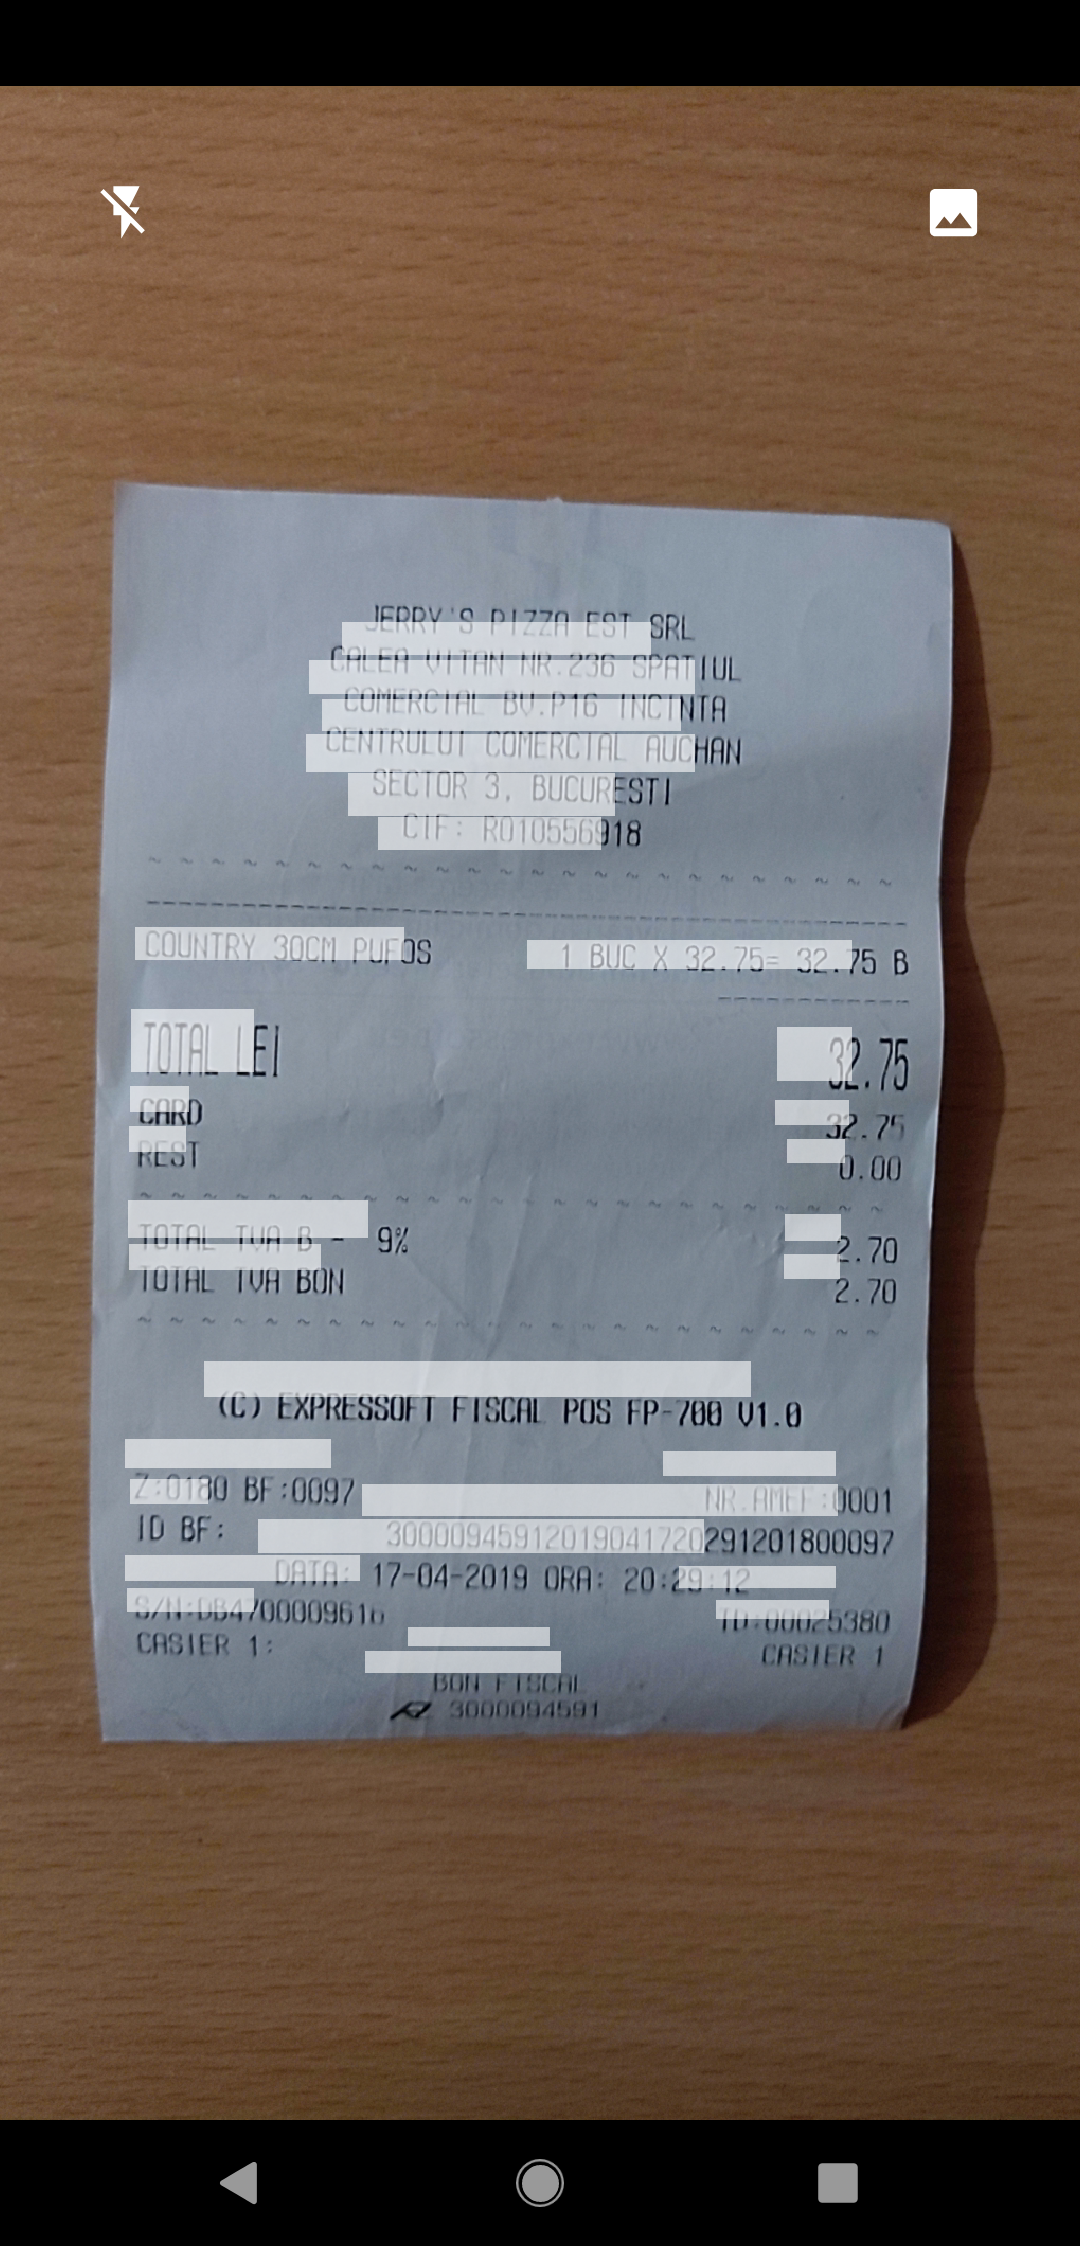
\includegraphics[width=0.25\textwidth]{Scanner.png}
%   \caption{Ecranul de Scanare}
%   \label{fig:scanner}
% \end{wrapfigure}
% \lipsum[1]


Aceasta este principala funcționalitate a aplicației și are ca scop extragerea informațiilor despre tranzacție dintr-o imagine cu un bon fiscal. Interfața cu utilizatorul este reprezentată de un vizor pentru camera principală a dispozitivului, ce afișează în timp real si textul detectat în imagine în spatele unor chenare.  Capturarea imaginii se face prin gestul \emph{tap} pe ecran. Funcționalitatea permite și folosirea unei imagini din galerie, dar și folosirea \emph{flash-ului} în condițiile de iluminare slabă. Odată capturată o imagine, procesarea acesteia se face pe un \emph{thread} secundar, în timp ce un ecran de încărcare este afișat. Figura \ref{fig:scanner} prezintă ecranul de scanare și chenarele de text recunoscute în imagine.

\begin{figure}[ht]
  \centering
  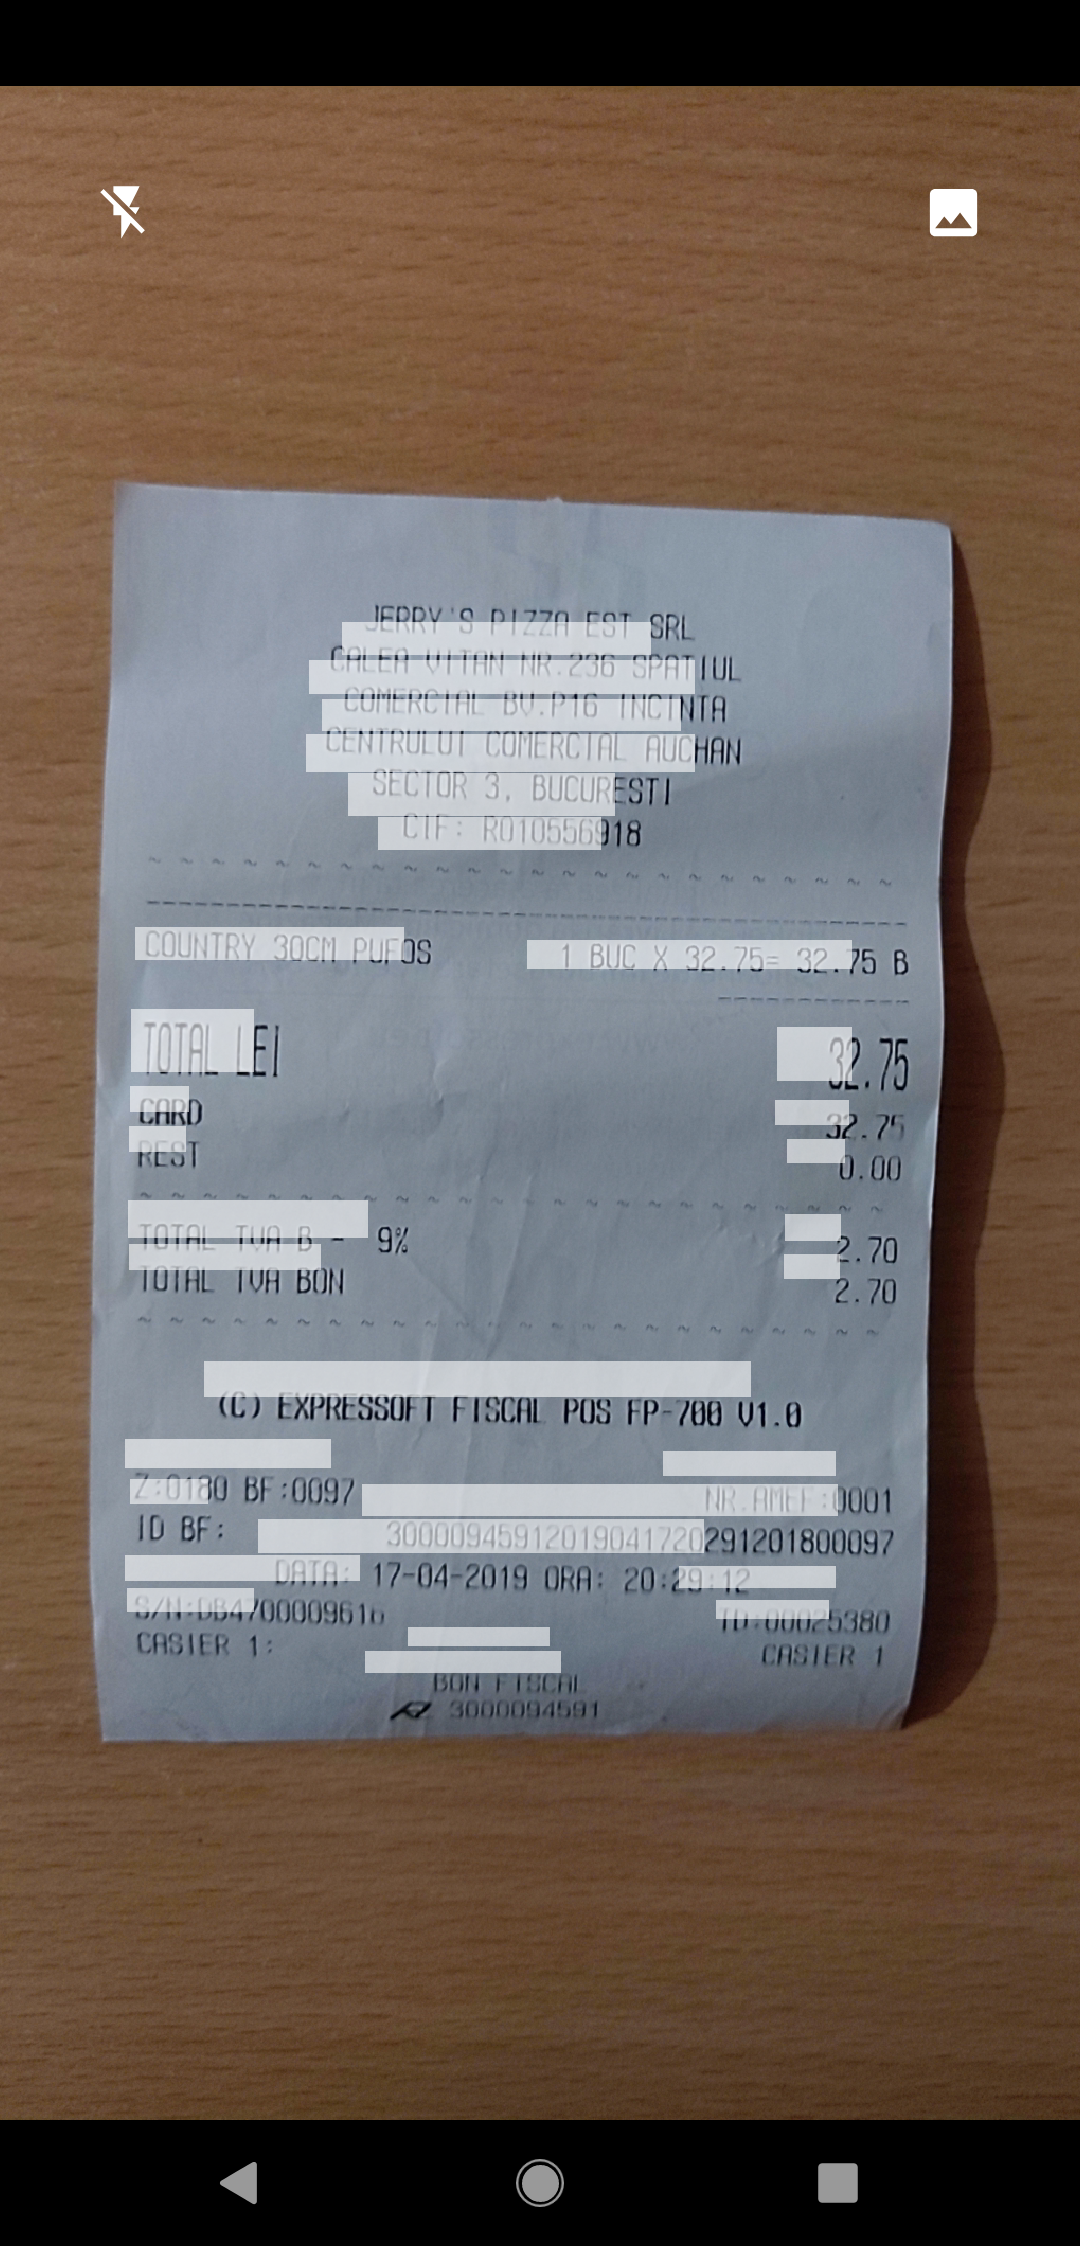
\includegraphics[width=\screenwidth]{Scanner.png}
  \caption{Ecranul de Scanare}
  \label{fig:scanner}
\end{figure}

\begin{itemize}
\item
  \textbf{Scop}: Capturarea unei imagini și extragerea informațiilor relevante din aceasta;
\item
  \textbf{Condiție de succes}: Prezența unei înregistrări în baza de date ce modelează bonul fiscal în starea de \emph{draft};
\item
  \textbf{Condiții de eșec}: Imaginea nu poate fi capturată; modulul OCR nu funcționează; o imagine este deja în curs de procesare;
\item
  \textbf{Precondiții}: Valorile predefinite pentru categorie și monedă;
\end{itemize}

\subsection*{Mențiuni}

Informațiile relevante de extras dintr-o imagine sunt:
\begin{multicols}{3}
\begin{itemize}
\item
  nume comerciant;
\item
  data tranzacției;
\item
  suma totală;
\item
  moneda;
\item
  categoria tranzacției;
\item
  produse:
  \begin{itemize}
  \item
    numele produsului;
  \item
    prețul aferent;
  \end{itemize}
\item
  elementele OCR:
  \begin{itemize}
  \item
    coordonatele casetelor de text;
  \item
    textul aferent;
  \end{itemize}
\end{itemize}
\end{multicols}

Imaginile se salvează astfel încât să nu fie accesibile din galerie.

\subsection*{Principalul scenariu}\label{principalul-scenariu}

\begin{enumerate}
\item
  Utilizatorul capturează o imagine;
\item
  Modulul OCR este apelat; Textul și chenarele aferente sunt extrase;
\item
  Rezultatul OCR este procesat pentru a obține conținutul bonului;
\item
  Bonul fiscal este salvat în stadiu de draft pentru a fi editat;
  (Specificație \ref{editare-draft})
\end{enumerate}

\begin{minipage}[t]{0.39\textwidth}
  \subsection*{Variații}\label{variaux21bii}
  \begin{itemize}
  \item
    Imaginea poate fi capturată utilizând camera telefonului sau importată
    din galerie;
  \item
    Moneda și categoria pot avea valori prestabilite, ce se modifică din setări; (Specificație \ref{spec:setari})
  \end{itemize}
\end{minipage}
\hspace{0.01\textwidth}
\begin{minipage}[t]{0.6\textwidth}
  \subsection*{Extensii}\label{extensii}
  \begin{itemize}
  \item
    Pentru a ajuta utilizatorul atunci când folosește camera, procesarea
    imaginilor venite de la cameră se face continuu, la o rată maximă
    configurabilă;
  \item
    Nu pot fi procesate mai multe imagini în același timp. Starea ultimei
    procesări este accesibilă permanent. Dacă se primește o cerere de
    procesare înainte ca ultima să se fi încheiat este semnalată o eroare.
  \end{itemize}
\end{minipage}


\section{Editare draft}\label{editare-draft}

Întrucât extragerea informațiilor nu este un proces robust, datele extrase trebuie validate de utilizator. Odată ce imaginile sunt procesate, datele extrase sunt salvate în baza de date, sub categoria \emph{drafts}. În acest moment, bonurile sunt editabile. Figura \ref{fig:draftList} prezintă ecranul unde utilizatorul vede toate drafturile, iar figura \ref{fig:draftScreen} ilustrează ecranul de editare.

\begin{figure}[!ht]
  \centering
  \begin{subfigure}{0.49\textwidth}
    \centering
    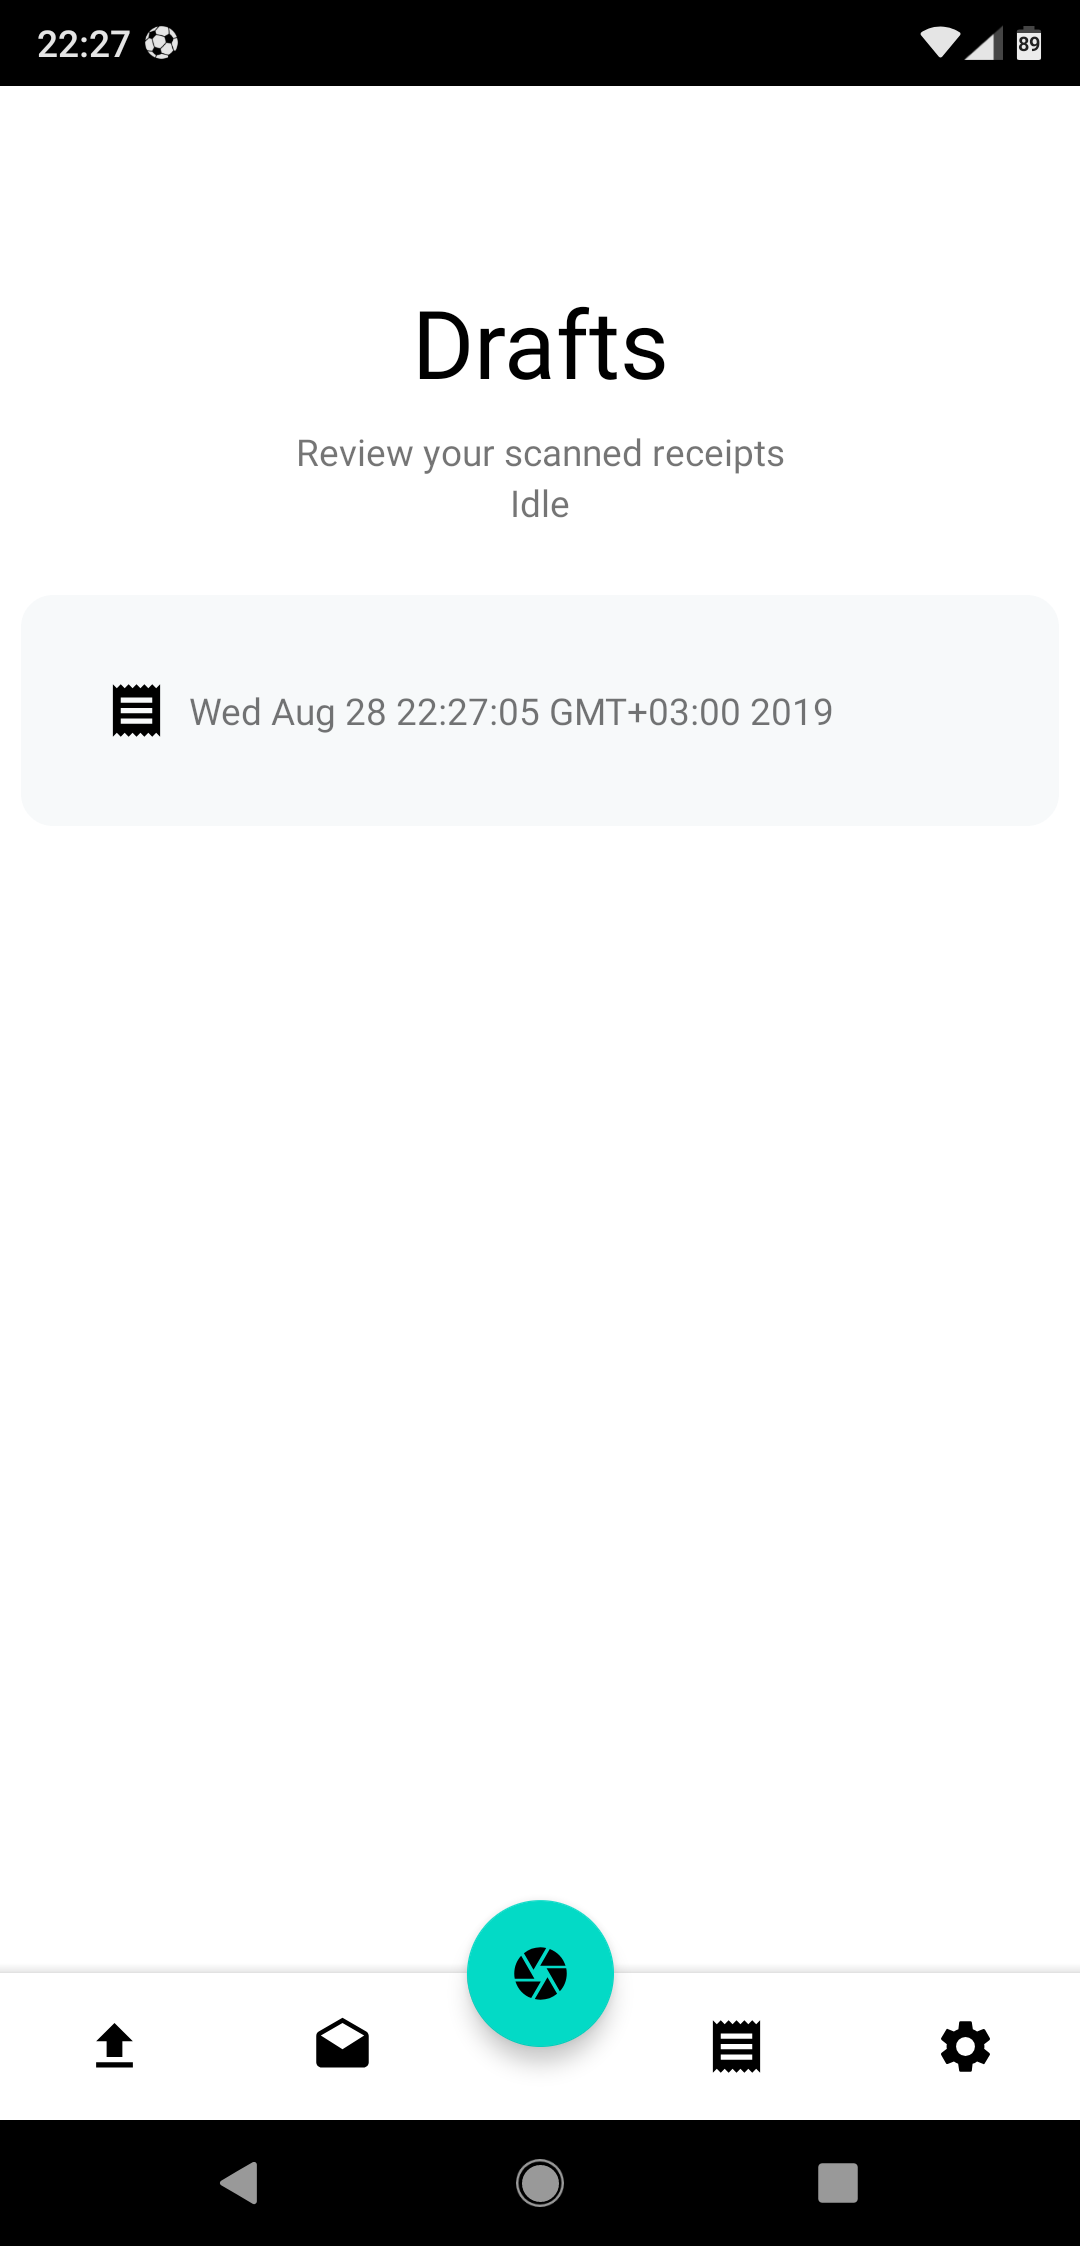
\includegraphics[width=\screenwidth]{DraftsList.png}
    \caption{Ecranul de listare}
    \label{fig:draftList}
  \end{subfigure}
  \begin{subfigure}{0.49\textwidth}
    \centering
    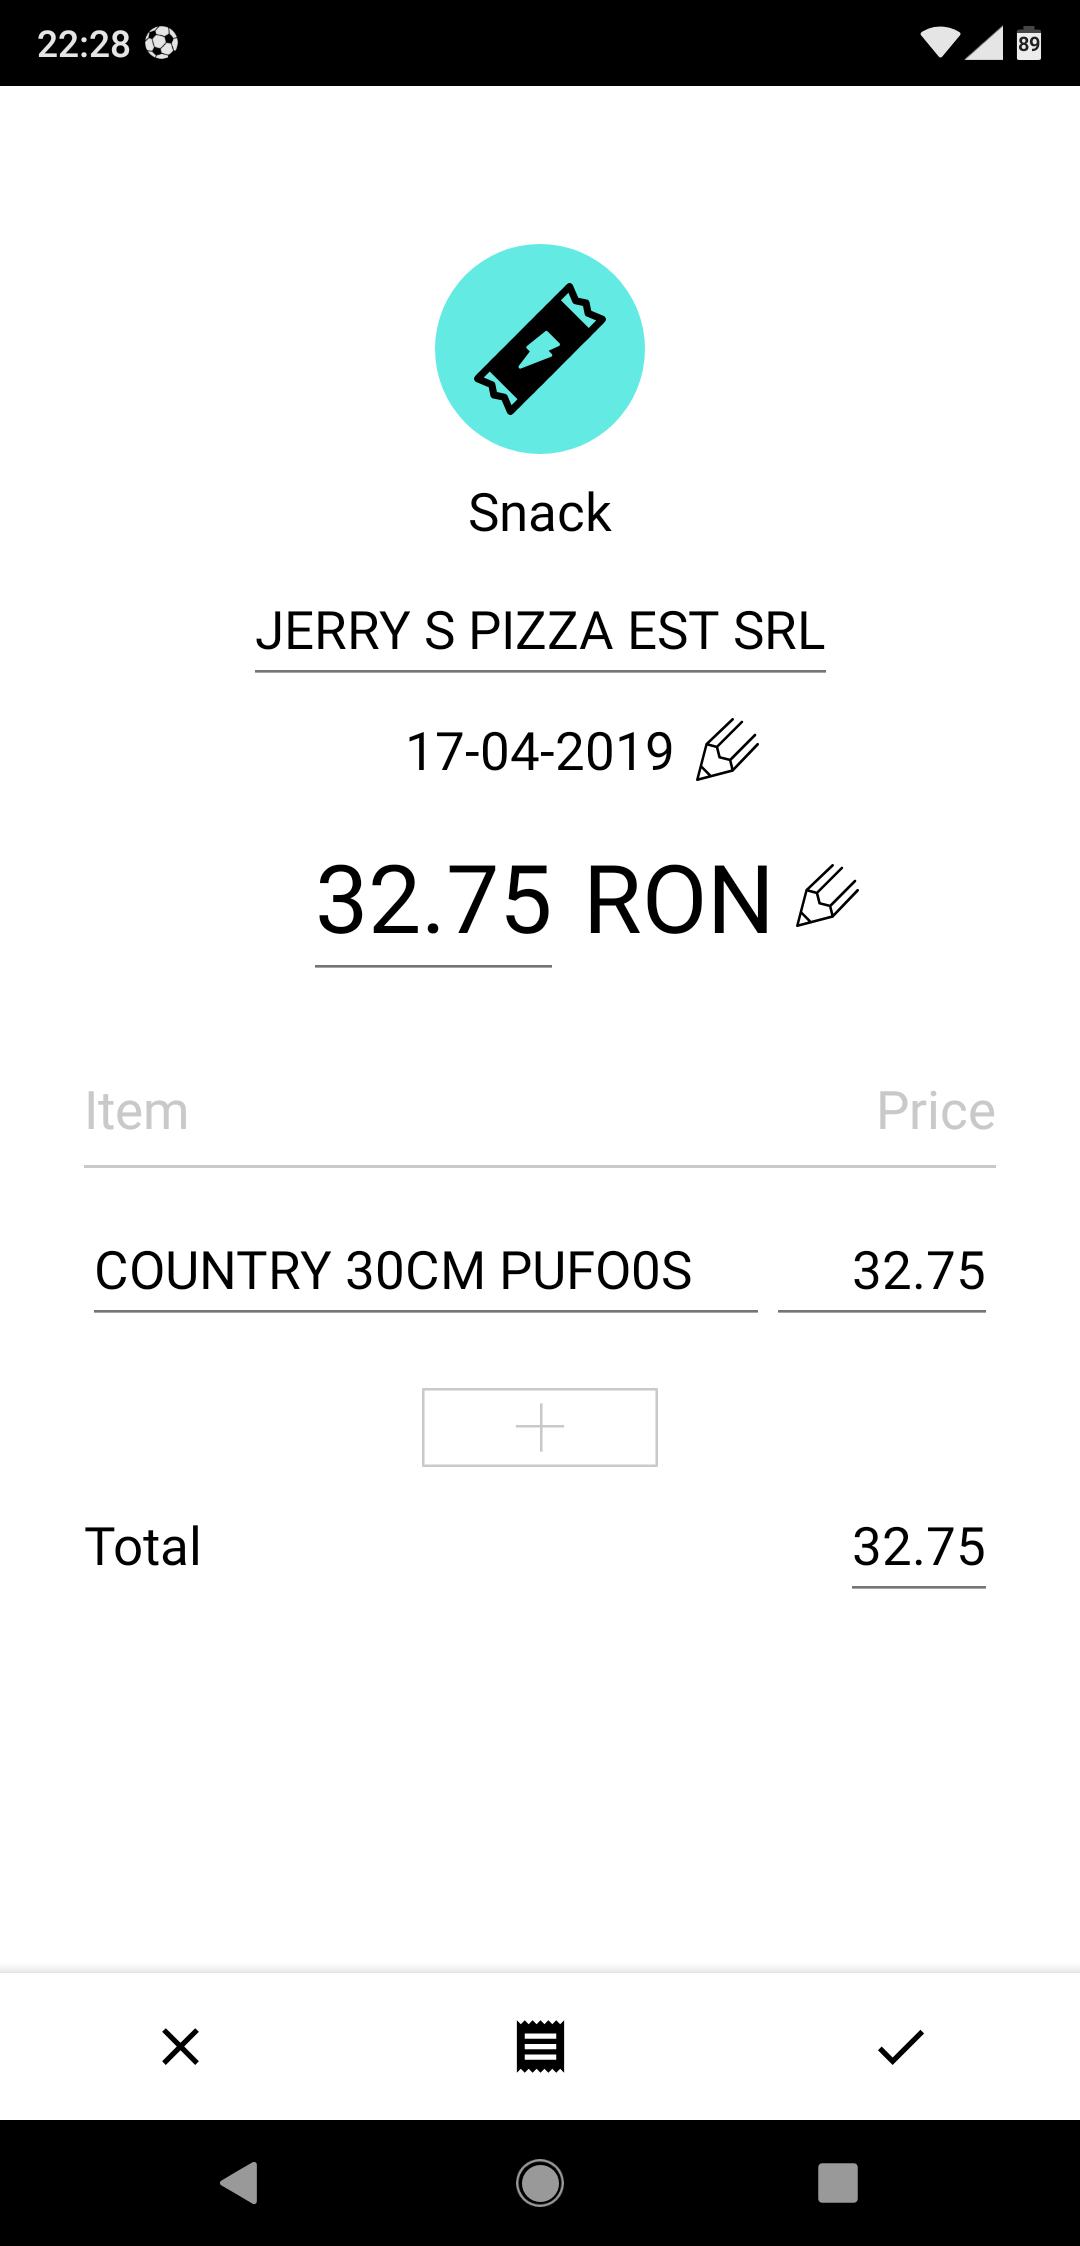
\includegraphics[width=\screenwidth]{DraftScreen.png}
    \caption{Ecranul de editare}
    \label{fig:draftScreen}
  \end{subfigure}
  \caption{Ecranele de gestionare a drafturilor}
  \label{fig:drafts}
\end{figure}

\begin{itemize}
\item
  \textbf{Scop}: Validarea informațiilor extrase din imagine de către utilizator;
\item
  \textbf{Condiție de succes}: Modificările făcute de utilizator se reflectă în baza de date; Bonul este validat și marcat ca final;
\item
  \textbf{Condiții de eșec}: Modificările nu pot fi persistate; Modificările sunt invalide;
\end{itemize}

\subsection*{Mențiuni}

Algoritmul de validare poate fi subiectul unor modificări ulterioare și trebuie să fie ușor de înlocuit.

Validarea considerată la momentul scrierii presupune ca niciun câmp să nu fie null sau fără conținut.

Asupra unui draft, utilizatorul are la dispoziție următoarele opțiuni:
\begin{multicols}{2}
\begin{itemize}
  \item
    modificarea categoriei, prin apăsarea pe ilustrația corespunzătoare;
  \item
    modificarea numelui comerciantului;
  \item
    modificarea datei, prin folosirea unui \emph{date picker};
  \item
    modificarea prețului total și a monedei;
  \item
    modificarea numelui sau prețului unui produs;
  \item
    ștergerea unui produs, prin gestul de \emph{swipe};
  \item
    adăugarea unui produs, prin apăsarea butonului de adăugare;
  \item
    ștergerea sau validarea \emph{draft-ului} și vizualizarea imaginii aferente prin butoanele din bara de opțiuni;
\end{itemize}
\end{multicols}

\subsection*{Principalul scenariu}


% \begin{minsipage}[t]{0.55\textwidth}

\begin{enumerate}
\item
  Utilizatorul accesează un bon;
\item
  Utilizatorul modifică câmpurile dorite;
\item
  Utilizatorul cere validarea bonului; Validarea se efectuează cu succes;
\item
  Bonul este scos din lista \emph{drafts} și pus în lista bonurilor validate;
\end{enumerate}

% \end{minipage} \vspace{0.01\textwidth}
% \begin{minipage}[t]{0.44\textwidth}

\subsection*{Variații}

\begin{itemize}
\item
  Utilizatorul poate modifica valori, dar fără a valida bonul;
\item
  Utilizatorul poate valida bonul, ceea ce îl scoate din lista de \emph{drafts} și îl pune în lista de bonuri valide;
\item
  Accesarea unui bon se face fie prin alegerea acestuia din listă, fie în urma scanării unei imagini; (Înțelegerea imaginilor)
\end{itemize}
% \end{minipage}
  
\subsection*{Extensii}

\begin{itemize}
\item
  Utilizatorul poate vedea imaginea capturată, cu și fără elementele OCR;
\item
  Utilizatorul poate vedea toate bonurile din lista \emph{drafts} și poate naviga către unul din ele;
\end{itemize}



\section{Gestionare setări}\label{spec:setari}

Aplicația permite setarea de valori predefinite pentru monedă și categorie, care să fie folosite în interpretarea imaginilor. De asemenea, aplicația permite activarea sau dezactivarea colectării de date în mod anonim (Specificația \ref{spec:collecting}). Figura \ref{fig:settingsScreen} prezintă ecranul de modificare a setărilor. 

\begin{figure}[h]
  \centering
  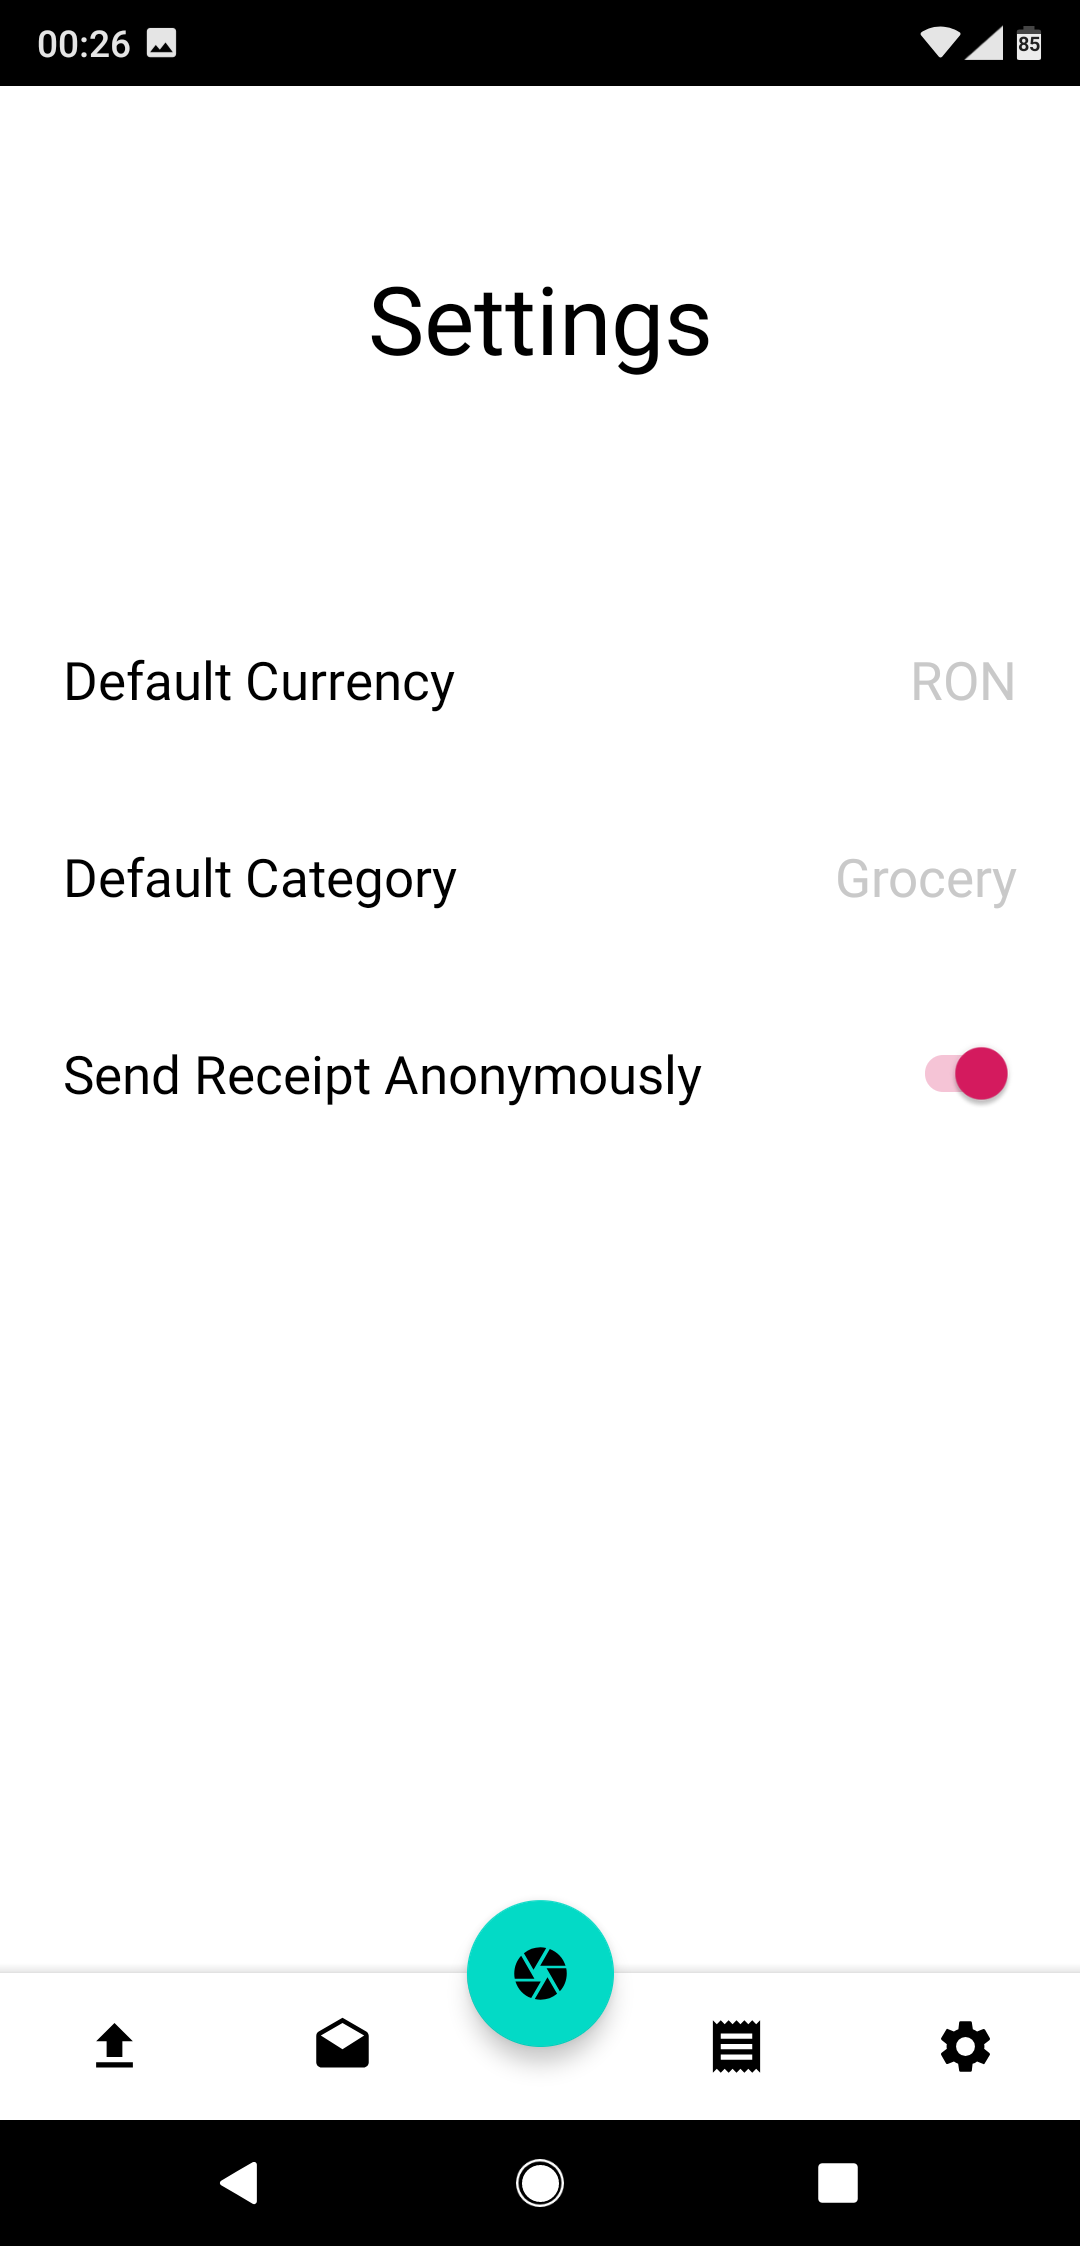
\includegraphics[width=\screenwidth]{SettingsScreen.png}
  \caption{Ecranul de setări}
  \label{fig:settingsScreen}
\end{figure}

\begin{itemize}
\item
  \textbf{Scop}: Modificarea și accesarea unor valori folosite în diferite puncte ale aplicației;
\item
  \textbf{Scenariu de succes}: Modificările făcute de utilizator sunt persistate și pot fi accesate;
\item
  \textbf{Scenarii de eșec}: Modificările nu pot fi persistate; Valorile nu pot fi accesate;
\end{itemize}

\begin{minipage}[t]{0.49\textwidth}

\section*{Mentiuni}
Setările considerate sunt:
\begin{itemize}
  \item
    Valoarea predefinită pentru categorie;
  \item
    Valoarea predefinită pentru monedă;
  \item
    Activarea sau dezactivarea colectării anonime de date;
\end{itemize}    

\end{minipage} \hspace{0.03\textwidth}
\begin{minipage}[t]{0.48\textwidth}
  
\subsection*{Principalul scenariu}
\begin{enumerate}
\item
  Utilizatorul accesează setările
\item
  Utilizatorul modifică valoarea unei setări;
\item
  Noua valoare este persitată și accesibilă;
\end{enumerate}  

\end{minipage}




\section{Colectarea bonuri fiscale}\label{spec:collecting}

Așa cum am menționat mai sus, această aplicație este construită având în vedere siguranța și confidențialitatea datelor. Totuși, lipsa de date care să facă legătura între imagini ale chitanțelor comerciale și conținutul acestora este un impediment în a rezolva problema în cauză prin metode avansate, care să ofere o performanță sporită. De exemplu, construirea unui astfel de set de date ar conduce la întocmirea unui \emph{benchmark} asupra căruia să fie testate noi metode. 

Astfel este motivată implementarea acestei funcționalități. Colectarea trebuie să se facă în \emph{mod anonim}, numai cu \emph{acordul utilizatorului} și să aibă un \emph{impact minim asupra experienței utilizatorului}.

\begin{itemize}
\item
  \textbf{Scop}: Utilizatorul salvează un bon, acesta este sincronizat în cloud numai dacă utilizatorul permite colectarea de date;
\item
  \textbf{Condiție de succes}: Bonul este trimis cu succes către server;
\item
  \textbf{Condiții de eșec}: Colectarea este permisă, utilizatorul salvează un bon, acesta nu este sincronizat în cloud; Datele nu pot fi accesate la momentul sincronizării;
\item
  \textbf{Precondiții}: Colectarea este permisă sau nu
\end{itemize}

\subsection*{Mențiuni}\label{menux21biuni-2}

Acțiunea de sincronizare se face în background, fără ca atenția utilizatorului să fie atrasă. Sincronizarea se face numai pe conexiune Wi-Fi și poate fi amânată până când conexiunea este disponibilă.

Se sincronizează toate informațiile aferente bonului, inclusiv imaginea și elementele OCR.

\subsection*{Principalul scenariu}\label{principalul-scenariu-3}

\begin{enumerate}
\item
  Utilizatorul finalizează salvarea unui bon cu succes;
\item
  În consecința acțiunii de salvare, precondiția este interogată;
\item
  Dacă este permisă colectarea, bonul este sincronizat în cloud;
\end{enumerate}

\section{Export}\label{export}

\begin{itemize}
\item
  \textbf{Scop}: Accesarea datelor în afara aplicației și a dispozitivului;
\item
  \textbf{Condiție de succes}: Utilizatorul selectează formatul, conținutul și perioada pentru export și primește un link la care poate accesa datele;
\item
  \textbf{Condiție de eșec}: Nu există date înregistrate în perioada selectată; Datele nu sunt trimise cu succes; Utilizatorul nu primește link-ul aferent;
\end{itemize}

\subsection{Mențiuni}\label{menux21biuni-3}

Pentru a consuma cât mai puține resurse (timp, baterie), exportul se face cu minim de procesare pe dispozitiv;

Datele salvate pe cloud au o dată de expirare, după care sunt șterse;

Odată ce datele sunt încărcate și procesate în cloud, aplicația primește o notificare ce conține link-ul de descărcare;

Datele pot fi descărcate într-o arhivă zip;

\subsection{Variații}\label{variaux21bii-2}

\begin{itemize}
\item
  Pentru a oferi maximum de flexibilitate utilizatorilor, datele pot fi accesate in format JSON sau CSV și pot conține fie doar text, fie text și imagini;
\end{itemize}

\subsection{Extensii}\label{extensii-2}

\begin{itemize}
\item
  În cazul lipsei de conectivitate, acțiunea de export este programată pentru o dată ulterioară, odată ce telefonul are conexiune;
\item
  Toate sesiunile de export sunt înregistrare într-o listă și sunt eliminate odată ce datele aferente sunt șterse din cloud;
\end{itemize}
